%!TEX root = ../LaTeX-cn.tex
\chapter{\tikzz\  绘图*(编写中,更新于\today)}
本章节极大地参考了 \tikzz\ 宏包手册\cite{tikzmanual}.
\section{\tikzz\ 简介}
``\tikzz \& PGF''(大多直接称为\tikzz)是 \LaTeX\ 上与 PSTricks(PostScript Tricks) 齐名的绘图扩展,而这两者基本上是在你的 \LaTeX\ 文档中绘制矢量图的唯二选择.Till Tantau\footnote{Till Tantau(1975---),德国吕贝克大学理论计算机科学研究处教授.他同时也是 \LaTeX\ 大名鼎鼎的幻灯片制作宏包 \pkg{beamer} 的开发者.} 开发了 \tikzz.

其中,``PGF'' 是 ``Portable Graphic Format''(便携图像格式)的缩写,是整个绘图系统的底层(或者后端);而 ``\tikzz'' 是 ``TikZ ist \emph{kein} 
Zeichenprogramm'' 的缩写,即英文的 ``TikZ is not a drawing program''(“\tikzz\ 不是绘图软件”),则是系统的前端.Till 是仿造 GNU 的缩写 ``GNU is Not Unix'' 这种递归式格式命名 \tikzz\ 的,他在文档中也提及了这一点.

从 \tikzz\ 发布稳定版以来,它的功能可以说涵盖了文档绘图的绝大部分\textbf{科学绘图场景}(我强调这一点,是因为我相信用它画艺术设计图的效率会很低)——对于研究工作者或者学生,这再好不过了.举个例子:笔者在大学期间的计算机和统计课程的所有出图都是由 \tikzz\ 绘制的.

\tikzz\ 的官方文档,使用\texttt{texdoc tikz}命令调出.看的出来,Till 努力将文档写的生动有趣.如果不是篇幅实在有些长,相信你读起来会很愉快.

\subsection{选择 \tikzz\ 还是 PSTricks}
关于这两者应该学哪一个,大家甚至展开圣战;虽然没有计算机行业 Vim 和 Emacs 圣战那么夸张,但是着实给不少想要学习 \LaTeX\ 绘图的人带来困扰\footnote{笔者就颇受困扰,所以都尝试过.当年还有人把 Asymptote 也扯进这场圣战,但笔者认为它的竞争力没有那么强.}.

笔者最后选择了 \tikzz\ .为什么?相比 PSTricks,语法顺畅,可读性更高.易读易写,十分难得.至于谁的绘图能力更强,我认为他们都已经涵盖了你正常需要的范畴.所以,如果你仍然不确定的话,就去搜索一些他们各自的例子片段再决定吧.

\subsection{选择 \tikzz\ 还是外部绘图软件}
为什么选择 \tikzz\ 而不是用外部绘图软件呢?一些理由:
\begin{itemize}
\item \textbf{绘制矢量图}.外部绘图为 pdf 矢量图再用加载图片的方式加载进来当然可以;但是很多情况下,切换软件的时间成本与切换到另一个软件的操作模式的思考成本是很高的.
\item \textbf{更小的体积}.相比加载外部绘图,体积会小一些;虽然不是特别明显.
\item \textbf{更易维护}.外部绘制的图片需要你通过安装相应的绘图软件进行维护;但是使用 \tikzz\ 绘图,你只需要一台装有 \LaTeX\ 核心和 \tikzz\ 宏包的设备.

千万别小看这一点;很多时候你需要在别人的电脑上更改你的插图.比如学术圈子里,电脑上安装有 \TeX\ Live 是一件稀松平常的事情;但是安装有 GNUplot 绘图,矢量图编辑器?那可不一定.
\item \textbf{完全的文本文件}.如果你使用 git 之类的版本控制工具,你应该会明白这一条是什么意思.不管你是将 \tikzz\ 代码写在主 tex 文档中,还是另存到一份单独的 tex 文档,它们都是文本文件.如果用加载外部 pdf 的方式导入图片,那想对它们进行版本控制简直是一场灾难.
\end{itemize}

\section{\tikzz\ 的输入输出}
\subsection{基本绘图方式}
\tikzz\ 的基本绘图方式有两种:使用 \latexline{tikz} 命令,或者使用 \envi{tikzpicture} 环境.请注意,\RED{语句用分号结尾}.当然,你需要先加载 \pkg{tikz} 宏包,有时你还需要加载一些 \tikzz\ 的库:
\begin{latex}
\usepackage{tikz}
% 加载库:\usetikzlibrary{lib1, lib2, ...}
\end{latex}

两个例子:
\begin{codeshow}
% 使用 \tikz 命令
\tikz{\draw (0,1) -- (1,0)}
% 使用 tikzpicture 环境
\begin{tikzpicture}
\draw (0,0) -- (1,1);
\end{tikzpicture}
\end{codeshow}

如果你使用 \TeX\ 而非 \LaTeX\ ,那么请在 \latexline{tikzpicture} 和 \latexline{endtikzpicture} 之中使用 \tikzz\ 代码.

\subsection{输出图像到独立文件}
要输出为\texttt{.svg}矢量文件,用于更多的插图场合.需要在电脑安装pdf2svg\footnote{\url{http://www.cityinthesky.co.uk/opensource/pdf2svg/}}.不过在\LaTeX 使用的场合,可以去掉下述的\texttt{convert}参数,以输出\texttt{.pdf}格式的矢量文件.下例中的\texttt{multi=false}表示只输出为单页文件.

\begin{latex}
\documentclass[tikz,convert=pdf2svg,multi=false]{standalone}
% tikz package already loaded by 'tikz' option
\begin{document}
\begin{tikzpicture}
  \draw (0,0) -- (10,10);
  \draw (10,0) -- (0,10);
\end{tikzpicture}
\end{document}
\end{latex}

在编译时如果是\xelatex ,还需要添加参数:
\begin{latex}
% 如果上例的文件名为 example.tex
xelatex -shell-escape example.tex
\end{latex}

\section{基础几何元素}
本节介绍 \tikzz\ 的基础几何元素,希望能够帮助读者较系统地进行学习.如果读者希望通过例子入手,请参考\secref{sec:tikz-eg}.

\subsection{点与线段}
点和线是绘图的基本要素.\tikzz\ 通过坐标的方式指定点的位置,坐标书写在一对圆括号内;通过两个短横线“--”来连接点与点,形成线段.下例连续画了两段.\RED{为了简洁,下文展示代码时省略 tikzpicture 环境首尾}.
\begin{tikzshow}
\draw (0,0) -- (1,0) -- (2,0.5);
\end{tikzshow}

默认的单位长度是 1 cm.如果想要修改比例尺,或者调整线型、颜色等属性参数,请参考\secref{sec:tikz-property}.极坐标参考\secref{subsec:polar}.

\subsection{路径}
命令 \latexline{path} 可以只创建路径但不绘制;实质上,\latexline{draw} 命令就是 \latexline{path[draw]} 的简写形式.\latexline{fill} 命令也类似.

\subsection{\bz\ 曲线}
\tikzz\ 允许你使用 \tikzkw{.. controls <p1> and <p2> ..} 方式来指定\bz\ 曲线的两个控制点.第二控制点可以省略;省略时,设为与第一控制点相同.
\begin{tikzshow}
\draw (0,0) .. controls (0.5,1) and (1.5,1) .. (2,0);
\end{tikzshow}

控制点并不会显式地画在图中.为了帮助不熟悉 \bz\ 曲线的读者理解,在此绘制一些辅助说明的点和线:
\begin{tikzshow}
\draw (0,0) .. controls (0.5,1) and (1.5,1) .. (2,0);
% Auxilary Points & Lines
\filldraw[black] (0,0) circle [radius=2pt] (0.5,1) circle [radius=2pt] (1.5,1) circle [radius=2pt] (2,0) circle [radius=2pt];
\draw[dashed] (0,0) -- (0.5,1);
\draw[dashed] (1.5,1) -- (2,0);
\end{tikzshow}

\subsection{矩形}
指定矩形的西南角点和东北角点,用 \tikzkw{rectangle} 命令连接:
\begin{tikzshow}
\draw (0,0) rectangle (2,1);
\end{tikzshow}

\subsection{圆与椭圆}
指定圆或者椭圆的中心,然后指明它半径的参数\footnote{\texttt{circle (1cm)} 的写法较陈旧,不建议再使用.椭圆绘制也请使用 \tikzkw{circle},而不是陈旧的 \tikzkw{ellipse}.}:
\begin{tikzshow}
\draw (0,0) circle [x radius=12pt, y radius=6pt];
\draw (2,0) circle [radius=0.5cm];
\end{tikzshow}
上例使用了 \tikzkw{rotate} 选项,绕原点(而非圆心)逆时针 30\(^\circ\) 旋转了椭圆.

\subsection{圆弧与椭圆弧}
指定圆弧的起点,在选项中给出起始角度、终止角度和半径,即可画弧:
\begin{tikzshow}
\draw (2,0) arc [start angle=0, end angle=45, radius=2];
\draw (1,0) arc [start angle=0, end angle=270, x radius=1, y radius=.5];
\end{tikzshow}
圆弧使用极坐标参数绘制往往更加简便,参考\secref{subsec:polar}.

\subsection{网格}
网格即为自动绘制的等距线:
\begin{tikzshow}
\draw[step=0.5,lightgray,thin] (0,0) grid (2,2);
\draw (1,1) circle [radius=.5];
\end{tikzshow}
默认的 \tikzkw{step} 是 1. \tikzkw{xstep} 和 \tikzkw{ystep} 命令可分别指定沿两个轴向的间距.

\subsection{抛物线*}
抛物线使用 \tikzkw{parabola} 绘制,并可使用 \tikzkw{bend} 指定拐点位置:
\begin{tikzshow}
\draw[help lines, xstep=1, ystep=2] (0,0) grid (3,4);
\draw (0,2) parabola[bend at end] (1,0);
\draw[xshift=1cm] (0,1) parabola (1,2);
\draw[xshift=2cm] (0,0) parabola bend (0.5,2) (1,0);
\draw[yshift=2cm] (0,0) parabola[bend pos=0.75] bend +(0,1) (1,0);
\draw[xshift=1cm, yshift=2cm] (0,0) -- (1,2) parabola cycle;
\draw[xshift=2cm, yshift=2cm] (0,0) parabola[parabola height=2cm] +(1,0);
\end{tikzshow}
其中 \tikzkw{xshift/yshift} 参考 \secref{subsubsec:shift}.抛物线的参数解释如下:
\begin{para}
\item[bend at end] 或者 \tikzkw{bend at start},这样抛物线是正常情况的一半.
\item[bend] 指定在何处设置拐点.
\item[bend pos=L] 在起点、终点连线的 L 分点处为基准设置拐点,比如上例为四分之三分点向上偏移 1 单位.
\item[cycle] 使用 \tikzkw{cycle} 结尾,自动直线连接首尾,形成闭合路径.
\item[parabola height=H] 在起终点连线的二分之一分点处向上偏移 H 处设置拐点.
\end{para}

\subsection{正弦线与余弦线*}
使用 \tikzkw{sin} 和 \tikzkw{cos} 绘制.

\section{坐标与图像}
\subsection{引言:画笔位置}
\tikzz\ 中一个很重要的概念是画笔,在一个常规的 \latexline{draw} 命令中,想象使用画笔从头到尾依次连接各个点.每次检测到“--”这条绘制命令,\tikzz\ 都将移动画笔位置并画线.

\tikzz\ 提供了一种方法,可以在移动画笔的同时不划线.这个命令就是 \tikzkw{++}:
\begin{tikzshow}
\draw (0,0) -- (1,0) ++(0,1) circle [radius=.25] -- ++(-1,0) -- (0,0);
\end{tikzshow}

\tikzz\ 还提供了一个命令 \tikzkw{+},可以\textbf{临时}偏移画笔:
\begin{tikzshow}
\draw (0,0) -- (1,0) -- +(0,1) circle [radius=.25] -- +(-1,1) -- +(-1,0);
\end{tikzshow}

请仔细体会两个命令的不同之处:单加号用于\uline{指代相对坐标},而相对坐标的基准点不会改变,直到指定新的绝对坐标 ;双加号用于\uline{移动画笔},基准点的位置会随之改变.

\subsection{极坐标}
格式是 \texttt{(角度:\mbox{}距离)}.
\label{subsec:polar}
\begin{tikzshow}
\draw (0,0) circle [radius=0.5] -- (30:1);
\end{tikzshow}

\subsection{交点}
\label{subsec:intersection}
\tikzz\ 提供一种简洁的坐标交点控制,例如 \texttt{(<p1> -| <p2>)} 中,用短横表示过 \texttt{p1} 的水平线、用竖线表示过 \texttt{p2} 的竖直线,这两条线的交点就是该命令表示的点.类似还有命令 \tikzkw{|-} .
\begin{tikzshow}
\draw (0,0) circle [radius=1cm] -- (30:1 |- 0,0) -- (30:1) -- cycle;
\end{tikzshow}

利用 \tikzz\ 的 \pkg{intersections} 库,还可以寻找两条路径的交点:
\begin{tikzshow}
% \usetikzlibrary{intersections}
\path[name path=line1] (0,0) -- (1,1);
\path[name path=line2] (0,1) -- (1,0);
\draw[name intersections={of=line1 and line2, by=A}] (0,0) -- (A) -- (1,0);
\end{tikzshow}

有时路径会有多个交点,这时你可以依次用 \texttt{intersection-1, 2, \ldots} 来指定它们.或者,你可以使用 \tikzkw{name} 选项代替上例的 \tikzkw{by},然后使用你的自定义名称:
\begin{tikzshow}
\path[name path=line1] (-2,.25) -- (2,.25);
\draw[name path=circle] (0,0) circle [radius=.5];
\draw[name intersections={of=circle and line1, name=A}] (1,0) -- (A-1);
\draw (0,0) -- (A-2);
\end{tikzshow} 

\subsection{图像变换}
\tikzz\ 的图像变换主要包括 4 种:平移、旋转、缩放与倾斜.

除了这 4 种变换以外,\tikzz\ 也允许你使用 \tikzkw{cm} 选项,通过输入变换矩阵来完成变换.传入 4 值 1 坐标 \texttt{cm=\{a,b,c,d,(p,q)\}},则点 \((x,y)\) 会被变换为 \((x',y')\):
\[
\begin{pmatrix} x' \\ y' \end{pmatrix} =
\begin{pmatrix} a & c\\ b & d \end{pmatrix}
\begin{pmatrix} x \\ y \end{pmatrix} + \begin{pmatrix} p \\ q \end{pmatrix}
\]
由于使用率极低,这里不再给出 \tikzkw{cm} 的例子;下面介绍 4 种主要变换.

\subsubsection{平移(shift)}
\label{subsubsec:shift}
在使用绘制命令时使用 \tikzkw{xshift}、\tikzkw{yshift} 或 \tikzkw{shift} 选项,可以平移路径.使用 \tikzkw{shift} 时,相对或绝对坐标都需写在花括号内.
\begin{tikzshow}
\draw (0,0) circle [radius=.5] -- (1,0);
\draw[xshift=1cm] (0,0) circle [radius=.5];
\end{tikzshow}

特别指出,\RED{平移是可以在路径的中间操作的,它只影响其后的绘制命令}:
\begin{tikzshow}
\draw (0,0) circle [radius=.5] [xshift=1cm, ultra thick] -- (0,0) circle [radius=.5];
\draw (.5,0) [shift={+(.5,.5)},->] -- (0,0);
\end{tikzshow}
上例使用了相对坐标,只把点 \((0,0)\) 变换成了点 \((1,.5)\).

另外,上例中的 \tikzkw{ultra thick} 影响了整个路径而不只是其后的部分,这也是 \tikzz\ 参数的一般情况;也就是说,平移参数不同于一般参数.

\subsubsection{旋转(rotate)}
 \tikzkw{rotate} 参数默认绕原点旋转.使用 \tikzkw{rotate around} 来指定旋转中心:
\begin{tikzshow}[scale=1.5]
\draw[lightgray] (0,0) rectangle (2,1)
    [rotate=15] (0,0) rectangle (2,1);
\begin{scope}[ultra thick]
\draw[blue] (.5,.5) rectangle (1.5,1); 
\draw[red] (.5,.5) [rotate around={45:(1,.5)}] rectangle (1.5,1); 
\draw[brown] (.5,.5) [rotate around={-60:+(.5,0)}] rectangle (1.5,1); 
\end{scope}
\end{tikzshow}
注意上例中相对坐标的使用,两次指定的旋转中心是同一个点.

旋转命令还可以用于三维坐标系中,例如使用 \tikzkw{rotate around x=<angle>} 来使绘图对象绕着 \(x\) 轴旋转.

\subsubsection{缩放(scale)}
使用 \tikzkw{xscale}、\tikzkw{yscale} 或 \tikzkw{scale} 选项,可以作为 \envi{tikzpicture} 环境的可选参数使用,也可以直接用在命令中:
\begin{tikzshowenvi}
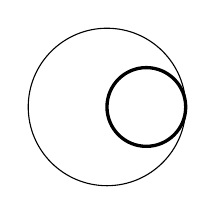
\begin{tikzpicture}[scale=.5]
\draw[very thick] (1,0) circle [radius=1];
\draw[scale=2] (0,0) circle [radius=1]; 
\end{tikzpicture}
\end{tikzshowenvi}
第二行的缩放 \texttt{scale} 是正常图像的 \(0.5\times 2=1\) 倍.

使用负值来实现“翻转”效果,以及使用 \tikzkw{scale around} 来指定缩放中心:
\begin{tikzshow}[very thick]
\draw[thin] (0,0) circle [radius=1];
\draw[xscale=-1] (0,0) rectangle (1,1);
\draw[red, xscale=-1] (0,0) rectangle (1,1);
\draw[blue, scale around={1.5:(1,1)}] (0,0) rectangle (1,1);
\end{tikzshow}

\subsubsection{倾斜(slant)*}
倾斜不是一个常用的图像变换.\tikzz\ 中的倾斜指令是 \tikzkw{xslant} 与 \tikzkw{yslant}.简单地解释,\texttt{xslant=k} 会把图像中坐标为 \((x,y)\) 的点变换为 \((x+k\times y, y)\).
\begin{tikzshow}[very thick,scale=.6]
\draw[help lines] (0,0) grid (4,2);
\draw (0,0) -- (1,1) -- (1,2) -- cycle;
\draw[red, xslant=1.5] (0,0) -- (1,1) -- (1,2) -- cycle;
\draw[blue, xslant=-1] (0,0) -- (1,1) -- (1,2) -- cycle;
\end{tikzshow}

\subsection{裁剪(clip)}
在 \latexline{clip} 命令\RED{之后}的所有绘图都会只显示该裁剪视窗中的部分:
\begin{tikzshow}
\clip (0,0) rectangle (1.1, 1.1);
\draw[red, thick] (0,0) circle [radius=1];
\end{tikzshow}

添加 \tikzkw{draw} 选项可以把 \latexline{clip} 命令的“轮廓”绘制出来\footnote{也可使用 \latexline{draw} 命令并将 \tikzkw{clip} 作为参数,还可将两者作为 \latexline{path} 命令的参数.}:
\begin{tikzshow}
\clip[preaction={draw=red,ultra thick}] (1.2,0) arc [start angle=0, end angle=225, radius=1.2];
\draw (-1,-1) rectangle (1,1);
\draw (-1,1) -- (1,-1);
\end{tikzshow}
上例使用一个非闭合的路径(圆弧)来裁剪,\tikzz\ 会自动将其首尾连接.其中,\tikzkw{preaction} 选项表示在 \latexline{clip} 命令\RED{之前}先沿该路径按传递给其的参数绘制,之后再创建裁剪视窗;这样可以实现视窗轮廓的自定义绘制(因为裁剪只影响其后的绘制命令).

\subsection{分组(scope)}
\label{subsec:scope}
分组操作允许你对当前组使用参数——这些参数会叠加到全局参数上,并且不影响到组外的对象:
\begin{tikzshowenvi}
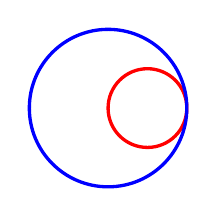
\begin{tikzpicture}[red, very thick, scale=.5]
\draw (1,0) circle [radius=1];
\begin{scope}[blue, scale=2]
\draw (0,0) circle [radius=1];
\end{scope}
\end{tikzpicture}
\end{tikzshowenvi}

\subsection{画布大小}
命令 \latexline{useasboundingbox} 可以

\section{点(node)与文本}

\subsection{点的坐标指定}
使用 \latexline{coordinate} 命令给点命名,便于之后引用.
\begin{tikzshow}
\coordinate (A) at (1,0);
\coordinate (B) at (1,1);
\draw (0,0) -- (A) circle[radius=.5] -- (B) -- cycle;
\end{tikzshow}
\tikzkw{coordinate} 也可以在绘制命令中作为选项使用.

\subsection{点的基本命令}
如需显式地绘制点(即占有面积的点),使用 \latexline{node} 命令,或者 \latexline{path} 命令的 \tikzkw{node} 选项.选项 \tikzkw{shape} 用于指定点的绘制方式.
\begin{tikzshow}
\node at (0,0) [shape=circle, draw] {a};
\node at (1,0) [rectangle, draw, fill=red] {};
\end{tikzshow}
选项 \tikzkw{shape} 还可赋值为 \texttt{coordinate},这样在点之间连线时会从点中心开始绘制,而不是从点的边框上,就像 \tikzkw{coordinate} 命令那样,是一个没有面积的“点”.

使用 \tikzkw{anchor} 选项定义对齐方式,可传入的值是东西南北(east, west, south, north)以及 4 个复合方位(south west).或者你可以依次用 left, right, above, below 来替代:
\begin{tikzshow}
\draw[help lines] (0,0) grid (2,2);
\draw (0,0) node [anchor=south west] {$\beta$};
\node at (0,1) [above right] {Here};
\node at (1,0) [above=2pt] {Hi};
\draw (1,2) node [below right=1pt and 8pt] {$1,0$};
\end{tikzshow}
其中,如果像最后一行给出双距离参数,需加载 \pkg{positioning} 库.

也可以直接用数字指定 \tikzkw{anchor} 的角度:
\begin{tikzshow}
\draw (0,0) circle [radius=1];
\foreach \x in {1,...,12} {
  \node at (90-30*\x:1) [anchor=270-30*\x] {\x};
}
\end{tikzshow}

点的命名类似 \latexline{coordinate} 的用法:
\begin{tikzshow}
\path node (a) at (0,0) {}
      node (b) at (1,0) {};
\draw (a) -- (b);
\end{tikzshow}

点的大小用 \tikzkw{inner sep} 指定文字到点边框的距离,用 \tikzkw{minimum size} 指定边框的最小尺寸.也可以配合 \tikzkw{text width} 选项指定文本的每行宽度.
\begin{tikzshow}
\tikzset{every node/.style={draw, circle}}
\node (a) {a};
\node[yshift=1cm] (b) {b};
\node[shift={(1,2)}, inner sep=2pt] (c) {c};
\node[xshift=1cm, minimum size=8pt] (d) {d};
\node[shift={(1,1)}, minimum size=8pt, inner sep=0pt] (e) {e};
\end{tikzshow}
注意点 \(d\) 和点 \(e\) 的区别.

\subsection{点的相对放置}
点的相对放置有两种方式.其一如下例,双距离语句需要 \pkg{positioning} 库.
\begin{tikzshow}
\tikzset{every node/.style={draw, circle}}
\draw[help lines] (0,0) grid (3,3);
\node (a) {a};
\node (b) [above=of a] {b};
\node (c) [above right=.5cm and 2cm of b] {c};
\node (d) [below=.5cm of c, on grid] {d};
\draw[red] (b) rectangle (d);
\end{tikzshow}
\tikzkw{on grid} 选项表示从边框而不是点中心开始计算距离,因此 \(b\) 与 \(d\) 的纵坐标不同.另一种方式是使用方位词结合点的名称,组成 \texttt{点名\mbox{.}方位词} 的语法:
\begin{tikzshow}
\node (a) {a};
\node[above] (aa) at (a.north) {a.north};
\end{tikzshow}
上例中的 \tikzkw{above} 选项不是必须的,但往往添加以避免点间的覆盖.

\subsection{点的旁置文本(label/pin)}
旁置文本(或标签)可用上一节的语法画另一个点来实现,但 \tikzkw{label} 或 \tikzkw{pin} 选项更简洁,会直接在主点旁画一个旁置点.对同一个主点画多个 \tikzkw{label} 或 \tikzkw{pin} 都是允许的;它们的区别在于后者会在主点和旁置点之间连一条线.

标签位置的语法是 \texttt{角度\mbox{:}文本}——它还有一个特殊的角度参数 \texttt{center},会将标签放在主点的中心处.你也可以通过 \tikzkw{label distance} 或 \tikzkw{pin distance} 选项来指定距离.
\begin{tikzshow}[every node/.style={draw, circle}]
\draw node[pin={[pin distance=.2cm, pin edge={<-, thick}]above right:$a_{p}$}] (a) at (0,0) {a} 
node[label={[red]30:$b'$}] (b) at (0,1) {b} 
node[label=120:$c'$, label=below:$c''$] (c) at (1.5,1) {c};
\end{tikzshow}
上例中甚至给 \tikzkw{label} 传入了颜色参数.还可以使用 \texttt{every pin, every pin edge} 或 \texttt{every label} 样式设定默认值.

当点被旋转时,参数 \tikzkw{absolute} 可以帮助你定位.如果它的值是 \texttt{true} 或缺省,那么方向不会跟随点而旋转,而是始终以纸面做参照:
\begin{tikzshow}
\tikzset{
    every node/.style={draw, rectangle},
    every label/.style={draw=red, font=\footnotesize}
}
\node[rotate=-80,label=right:label] (a) at (0,0) {normal};
\draw[blue, thick] (0,0) -- (-80:1);
\node[rotate=-80,label={[absolute]right:label}] (b) at (1,0) {absolute};
\draw[blue, thick] (1,0) -- +(0:1);
\end{tikzshow}
左侧标签的锚点(位于红色矩形的左侧边上)在点“normal”右侧边框的中点,而右侧标签的锚点则位于穿过点“absolute”中心的水平向右的线上.\RED{上例中出现了方括号嵌套时,不要忘记添加花括号}.

\subsection{点的沿路径文本}
\subsubsection{显示指定}
将 \tikzkw{node} 选项放于对应的点坐标之后,称为显示(explicitly)指定.

对于沿路径的文本标记,\tikzz\ 预定义了 7 种位置,分别是 \tikzkw{at start/end}, \tikzkw{(very) near start/end},以及缺省时的 \tikzkw{midway}.
\begin{tikzshow}
\draw (0,0) .. controls (.5,2) ..
  node[at start] {at start}
  node[sloped, above] {midway}
  node[pos=1, right, text width=3ex] {at end} (1.5,2);
\end{tikzshow}
上例中的一些参数:
\begin{para}
\item[sloped] 设置文字基线与图中此处的切线平行.
\item[pos] 定量化的位置参数\footnote{并不是严格的空间分点;而是基于首、尾、控制点间向量计算出速度,取其时间分点.很难精确指定.}.比如预定义的 \tikzkw{very near start} 即为 \(0.125\),\tikzkw{near start} 即为 \(0.25\).
\end{para}

对于交点指定(\tikzkw{|-} 或 \tikzkw{-|}),中点(\tikzkw{midway})即为垂足:
\begin{tikzshow}
\draw (0,0) |- (2,1) \foreach \p in {0,0.5,1} {
  node[pos=\p] {\p}
};
\end{tikzshow}

不同位置放置文本的场合,使用 \tikzkw{auto} 选项,并可以设定 \texttt{left} 或者 \texttt{right} 参数;选项 \tikzkw{swap} 则允许你将其文本放在对称位置.注意:这两个选项\RED{只对沿路径的放置有效}.
\begin{tikzshow}[scale=.5, every node/.style={circle, inner sep=2pt}]
\foreach \x in {1,...,4} {
  \draw (90-90*\x:2) -- (-90*\x:2)
  node[midway, fill=red!30, auto=left] {\x}
  node[midway, fill=blue!30, auto, swap] {\x};
}
\end{tikzshow}

\subsubsection{隐式指定}
路径中点的位置可以隐式(implicitly)指定,放在 \texttt{--} 命令与要连接的点之间(即可.只有隐式指定的点才会继承全局参数.例子\cite{tikzmanual}:
\begin{tikzshowenvi}
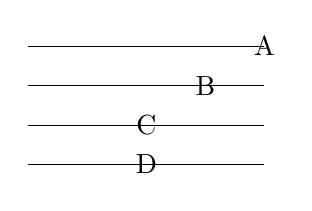
\begin{tikzpicture}[near end]
\draw (0,2.5) -- (3,2.5) node{A};
\draw (0,2) -- node{B} (3,2);
\draw (0,1.5) -- node[midway] {C} (3,1.5);
\draw (0,1) -- (3,1) node[midway] {D} ;
\end{tikzpicture}
\end{tikzshowenvi}
将上述代码中的 \tikzkw{--} 换成 \tikzkw{to} 也可以;通常后者是个更强的命令,在下一节中也会介绍.

\subsection{点之间的连线}
\subsubsection{基础连线}
点之间连线会自动检测点的绘制边界,主要要三种操作方式:
\begin{enumerate}
\item 在点名称后增加小数点和方位词来指定,比如点 a 的左侧就用 \texttt{(a.west)};
\item 使用 \texttt{to} 代替 \texttt{--},并附加 \tikzkw{out} 与 \tikzkw{in} 选项.(如果不附加则会画直线)
\item 使用 \texttt{to} 附加 \tikzkw{bend left/right} 选项.下例中最后一行以 a 到 b 直线方向为角度 0,\texttt{bend left=45} 表示逆时针旋转 $45$ 度作为 \tikzkw{out} 值,旋转 $180-45=135$ 度作为 \tikzkw{in} 值.
\end{enumerate}
\begin{tikzshow}
\tikzset{every node/.style={draw,circle}}
\node (a) {a};
\node (b) [below=of a] {b};
\node (c) [left=of b] {c};
\draw[blue, ->] (c.north) .. controls +(up:1) and +(left:1) .. (a.west); 
\draw[red, ->] (c) [out=315, in=225] to (b);
\draw[->] (a) to [bend left=45] (b);
\end{tikzshow}

\subsubsection{边命令(edge)}
边命令用于绘制包含同一个点的所有边.当你想要给每个点的边进行定制时,这会十分有用:
\begin{tikzshow}
\tikzset{every node/.style={draw,circle}}
\node (a) {a};
\node (b) [below=of a] {b};
\node (c) [left=of b] {c};
\draw[thick] (c) edge[red, -latex] (b)
    edge[bend left=45] (a)
    edge[blue, <-] (a);
\end{tikzshow}
提醒一下那些熟悉图论的读者:别忘了尽管最后一行中边的箭头方向是从 a 到 c 的,但仍可以像上面一样用 c 点的 \tikzkw{edge} 命令来绘制.

你还可以连写边命令,并沿边加上文字:
\begin{tikzshow}
\node foreach \name/\angle in {a/0,b/90,c/180,d/270}
    (\name) at (\angle:1.5) {$\name$};
\path[->] (b) edge node[above right] {$5$} (a)
  edge (c)
(c) edge [-,dashed, blue] node[auto] {auto}
  node[auto, swap] {swap} (a)
  edge (d)
(d) edge [red] node[above,sloped] {very}
  node[below,sloped] {red} (a);
\end{tikzshow}
这里用到了之前提及的 \tikzkw{auto} 命令.

\subsection{作为图像的点(pic)*}
一段绘图代码可能需要复用;如果它比较复杂,可以使用 \latexline{pic} 来重复调用.
\begin{tikzshow}[scale=0.8]
\tikzset{dcircle/.pic={\draw (0,0) circle [x radius=.5, y radius=.8] circle [radius=1];}}
% 两种调用方式
\draw[help lines] (0,-1) grid (2,2);
\pic at (0,0) {dcircle}; 
\path (2,0) pic {dcircle};
\end{tikzshow}
语法非常类似 \tikzkw{node}.其中 \tikzkw{at} 也可以写成 \texttt{[at=\{(0,0)\}]} 这种形式.

\tikzkw{pic actions} 选项用于传入 \texttt{draw, fill, shade, 或 clip} 参数:
\begin{tikzshow}[scale=0.6, transform shape]
\tikzset{circlerect/.pic = {
    \path[pic actions] (.5,.5) circle [radius=.3];
    \draw (0,0) rectangle (1,1);
}}
\draw[red] (0,0) grid (4,2);
\pic [blue, thick] at (.5,.5) {circlerect};
\pic [draw=blue, fill=white] at (2.5,.5) {circlerect};
\end{tikzshow} 
当不传入 \tikzkw{draw} 选项时,圆的 \latexline{path} 命令是不会绘制的;同时注意,因为绘制矩形的是 \latexline{draw} 命令,因此不受\tikzkw{fill} 选项影响.

插入的 \tikzkw{pic} 中的点可以在外部调用,一个例子:
\begin{tikzshow}
\tikzset{mypic/.pic={
  \draw[blue] (0,0) coordinate (-A)
  -- (1,1) coordinate (-B);
}}

\draw[help lines] (0,0) grid (1,2);
\pic (P) {mypic};
\pic (Q) at (0,1) {mypic};
\draw[red] (P-A) -- (Q-B);
\end{tikzshow}
\tikzkw{pic} 定义时用短横命名是为了可读性.调用时语法类似 \tikzkw{node}.

\pkg{quotes} 库支持以加引号字串的方式传入参数,作为 \tikzkw{pic text} 选项的值.比如 \texttt{angles} 这个预定义的 \tikzkw{pic}(由 \pkg{angle} 库支持):
\begin{tikzshow}
\draw (0,-1) coordinate (P1)
  -- (0,0) coordinate (O)
  -- (1,1) coordinate(P2)
  pic [draw, "$\alpha$"] {angle=P1--O--P2};
\end{tikzshow}

一些其他注意:
\begin{feai}
\item 如果有 \texttt{foreach} 语句,\textbf{请放在 \texttt{pic} 定义的首行} .
\item \tikzkw{pic} 虽说从用法上近似 \tikzkw{node},实质上它是以类似 \tikzz\ \envi{scope} 环境的方式工作的.因此,如果想要其外部的图像变换对其生效,须添加 \tikzkw{transform shape} 选项于 \envi{tikzpicture} 环境.
\item \tikzkw{pic} 对象也能像 \tikzkw{node} 一样,沿路径放置,设置 \tikzkw{at start} 等选项.
\item 将 \tikzkw{pic} 作为选项使用时,添加 \tikzkw{behind path} 或者 \tikzkw{in front of path} 来指定将 \tikzkw{pic} 插入到所在路径的下方或是上方图层.
\item 如果你只是临时使用而不想额外定义,这里有一个使用 \tikzkw{code} 选项的例子\cite{tikzmanual}:
\begin{tikzshow}
\draw (0,0) .. controls(1,0) and (2,1) .. (3,1)
foreach \t in {0, 0.1, ..., 1} {
  pic [pos=\t] {
    code={\draw circle [radius=2pt];}
  }
};
\end{tikzshow}
注意,本例只有一句语句.句中 \tikzkw{pic} 是 \latexline{draw} 命令的选项.
\end{feai}

\section{几何绘制}
严格的几何学绘图需要一些特别的命令,比如计算两点间的距离.而且,通常会使用 \tikzkw{coordinate} 而不是 \tikzkw{node} 命令;因为前者并不占用面积,这样画线时才能保证抵达点所在的中心坐标.

\subsection{坐标计算}
库 \pkg{calc} 允许用户使用 \texttt{(\$ ... \$)} 的形式来计算坐标:
\begin{tikzshow}
\coordinate[label=below:A] (A);
\coordinate[above right=.5 and 1.5 of A, label=right:B] (B);
\draw (A) -- (B);
\draw ($ (A) + (.3,.4) $) circle (.5);
\end{tikzshow}

\subsection{两点距离计算}
上一节中的半径值是人工计算的.下例让 \tikzz\ 计算距离,并用 \tikzkw{let} 选项将其储存起来,在 \tikzkw{in} 选项的后方进行调用:
\begin{tikzshow}[scale=0.6, transform shape]
\coordinate[label=left:A] (A);
\coordinate[above right=.5 and 1.5 of A, label=right:B] (B);
\draw (A) -- (B);
\draw let \p1 = ($ (B) - (A) $),
         \n{rad} = {veclen(\x1,\y1)}
    in (B) circle[radius=\n{rad}]
       (A) circle[radius=\n{rad}];
\end{tikzshow}
命令 \verb|\p<数字>| 用于存储向量计算结果,比如 \verb|\p1|.对应的,使用 \verb|\x1| 或者 \verb|\y1| 可以调用向量的两个坐标值.而 \verb|\n<数字>| 则用于存储数值.此外,命令 \tikzkw{veclen} 用于计算向量的欧式长度 \(\sqrt{x^2+y^2}\).  

如果不想使用数字命名,可以像上例的存储数值一样使用字符串;不过这样命名需要加上花括号.事实上,已知圆心 $A$ 和圆周上一点 $B$,有更简单的画圆方法,参考\secref{subsec:circlethrough}部分的内容.

\subsection{等分点}
等分点是几何中常用的概念,\pkg{calc} 库支持像 \pkg{xcolor} 混合颜色类似的命令:\verb|<点A>!<分点值>!<点B>|.而且它还可以用最后一行中链式的方法进行连写:
\begin{tikzshow}
\coordinate[label=left:A] (A);
\coordinate[above right=.5 and 1.5 of A, label=right:B] (B);
\coordinate (X) at ($ (A)!0.5!(B) $);
\coordinate[label=above:C] (C) at ($ (X)!{sqrt(3)}!90:(B) $);
\path[draw=black, fill=blue!20] (A) -- (B) -- (C) -- cycle;
\node[draw=black, fill=red!20, circle through=(X)] at ($ (A)!0.5!(B)!{tan(30)}!90:(B) $) {};
\end{tikzshow}
注意分点值如果需要计算(比如上例的根号),需要放在花括号内.

\subsection{过某点的圆*}
\label{subsec:circlethrough}
使用 \pkg{through} 库可以方便地画出给定圆心和过某点的圆,而不需要做两点距离计算:
\begin{tikzshow}[scale=0.75]
\coordinate[label=left:A] (A);
\coordinate[above right=.5 and 1.5 of A, label=right:B] (B);
\draw (A) -- (B);
\foreach \c/\r in {A/B, B/A}
  \node[draw,circle through=(\r)] at (\c) {};
\end{tikzshow}
注意,\tikzkw{circle through} 仅仅适用于 \tikzkw{node} 命令.

\subsection{交点}
在\secref{subsec:intersection}中已经介绍过交点的基本使用,包括 \tikzkw{-|} 指令与 \pkg{intersections} 库的一些用法.这里的例子更复杂一些,也复习了之前等分点的用法:
\begin{tikzshow}
\tikzset{small/.style={draw, circle, fill=black, inner sep=1pt}}
\coordinate[label=left:A] (A);
\coordinate[above right=.5 and 1.5 of A, label=right:B] (B);
\coordinate[label=below:C] (C) at ($ (A)!0.5!(B) $);
\coordinate (D) at ($ (C)!2!90:(B) $);
\coordinate (E) at ($ (C)!2!-90:(B) $);
\draw (A) -- (B);
\draw[red, name path=Lv] (E) -- (D);
\node[draw, circle through=(B), name path=Ca] at (A) {};
\path[name intersections={of=Lv and Ca, by={[label=above right:D]D, [label=right:E]E}}];
\foreach \x in {A,C,D,E}
  \node[small] at (\x) {};
\end{tikzshow}
注意上例中的 \latexline{path} 命令虽声明了交点,但没有画任何内容.

\section{属性}
\label{sec:tikz-property}

\subsection{线宽}
\tikzz\ 预定义了 7 种线宽,从细到粗是:\tikzkw{ultra thin}, \tikzkw{very thin}, \tikzkw{thin}, \tikzkw{semithick}, \tikzkw{thick}, \tikzkw{very thick}, \tikzkw{ultra thick}.或者利用 \tikzkw{line width} 选项指定.
\begin{tikzshow}
\draw[ultra thin] (0,0) -- (1,0);
\draw[ultra thick] (1,0) -- (2,0);
\draw[line width=10pt] (0,1) -- (2,1);
\end{tikzshow}

\subsection{线型}
\tikzz\ 预定义了 4 种基本线型:\tikzkw{dashed}, \tikzkw{dotted}, \tikzkw{dash dot}, \tikzkw{dash dot dot}.它们还可以配合 \tikzkw{loosely} 或者 \tikzkw{densely} 进行微调.
\begin{tikzshow}
\draw[dashed] (0,0) -- (1,0);
\draw[dotted] (0,-0.5) -- (1,-0.5);
\draw[dash dot] (0,-1) -- (1,-1);
\draw[dash dot dot] (0,-1.5) -- (1,-1.5);
\draw[loosely dashed] (0,-2) -- (1,-2);
\draw[densely dotted] (0,-2.5) -- (1,-2.5);
\end{tikzshow}

如果的确需要深度自定义,请使用 \tikzkw{dash pattern} 自定义线型,并可配合 \tikzkw{dash phase} 指定线型的起始位置.
\begin{tikzshow}
\draw[dash pattern=on .1cm off .25cm on .25cm off .15cm, dash phase=1cm] (0,0) -- (3,0);
\end{tikzshow}

有时你可能会看到一些复杂的装饰线(需要 \pkg{decorations} 库),比如:\tikz{\draw [->,decorate,decoration=snake] (0,0) -- (2,0)}.请参考\secref{subsec:deco}.

\subsection{箭头}
\tikzz\ 中的箭头多到可以单独开一个章节,但我并不想全部详尽地介绍.用大于或小于号表示箭头的指向,用竖线表示是否加上截断符号.一些基本的样例:
\begin{tikzshow}
\draw[->|] (1,3) -- (2,3);
\draw[stealth-] (1,2) -- (2,2);
\draw[->,>=stealth, line width=3pt] (1,1) arc [start angle=90, end angle=30, radius=1];
\draw[<->] (.5,4) -- (.5,0) -- (2.5,0);
\end{tikzshow}
其中,用 \texttt{>=stealth} 或 \texttt{-stealth} 的方式指定了箭头末端的类型为 \texttt{stealth}.你也可以将前者作为整个 \envi{tikzpicture} 环境的可选参数进行传递.

\tikzz\ 的 \pkg{arrows.meta} 库包含很多箭头,读者可以自行查阅.

\subsection{绘制颜色}
在绘制网格一节,已经使用过 \texttt{lightgray} 作为网格的绘制颜色;当时省略了 \tikzkw{draw} 选项.以下使用浅红色作为绘制色:
\begin{tikzshow}
\draw[draw=red!50!white, ultra thick] (0,0) rectangle (1,1);
\end{tikzshow}
其中,双感叹号加数字是表示插值比例为 0.5;\pkg{xcolor} 宏包支持该语法.在 \tikzz\ 环境内部,还可以使用 \latexline{colorlet} 命令自定义,例如:
\begin{latex}
\colorlet{linecolor}{red!60!black}
\end{latex}

\subsection{单色填充}
填充命令 \latexline{fill} 只能使用于闭合区域,\textbf{且不绘制区域边界}.你可以在一般绘制命令的末尾添加 \tikzkw{cycle} 来创建一个闭合对象:
\begin{tikzshow}
\fill[green] (0,0) -- (1,0) -- (1,1) -- cycle;
\end{tikzshow}

在填充的同时绘制\footnote{准确地说,\latexline{filldraw} 命令是先绘制再填充.},使用 \latexline{filldraw} 命令,并分别指定绘制和填充颜色:
\begin{tikzshow}
\filldraw[draw=black, fill=cyan] (0,0) -- (2,0) arc (0:30:2);
\end{tikzshow}

利用区域的奇偶性填充,使用 \tikzkw{even odd rule}:
\begin{tikzshow}
\fill[even odd rule, blue] (0,0) -- (2,0.5) -- (1,1) circle (0.25);
\end{tikzshow}

\subsection{渐变填充*}
使用 \latexline{shade} 命令控制渐变填充,

\section{样式与高级控制}
\subsection{样式(style)}
如果某种属性需要用来反复作图,可以把它自定义为样式:

上文中出现过的 \texttt{help lines},就是 \tikzz\ 预定义的一种样式.其相当于于:
\begin{latex}
\begin{tikzpicture}[help lines/.style={line width=0.2pt,gray}]
...
\end{tikzpicture}
\end{latex}

你也可以在进入 \tikzz\ 环境后(或在文档导言区),使用 \latexline{tikzset} 命令来定义.

\subsection{循环语句}
\tikzz\ 支持循环语句,这一点对于科技绘图来说十分重要.
\begin{tikzshow}[place/.style={circle, draw, fill=black, minimum size=5pt, inner sep=0pt}]
\foreach \x in {1,2,3} {
    \node at (\x, 0) [place] {};
    \draw (\x, 0) circle [radius=1/\x];
}
\end{tikzshow}

有时候我们需要循环一个等差数列,这时候使用 \ldots\ 即可.\tikzz\ 会将 \(a,b,\ldots,c\) 识别为从 \(a\) 到 \(c\) 以 \(b-a\) 为公差的等差数列;如果你不指定 \(b\),那么默认以 \(1\) 为公差.
\begin{tikzshow}[place/.style={circle, draw, fill=black, minimum size=5pt, inner sep=0pt}]
\foreach \x in {1,1.5,...,3,4} {
    \node at (\x, 0) [place] {};
    \draw (\x, 0) circle [radius=\x/8];
}
\end{tikzshow}
上例中的 \(4\) 不在数列内,这样写是允许的.数列后也可以接另一个数列.

大部分需要知道“循环到列表第几个”的场合,都可以配合移动画笔或相对坐标命令实现:
\begin{tikzshow}[scale=.5]
\draw[red] (0,0) grid (3,3);
\foreach \x/\y in {0,1/2,2}
  \draw (\x, \y) +(.5,.5) circle [radius=.4];
\end{tikzshow}
上例同时循环了多个变量,中间用斜线分隔;它们分别按照列表中斜线分隔后的对应值进行循环.如果某一位置的列表提供值的个数小于变量的个数,那么“多出”的变量将都取最后一个值.

此外,如果 \latexline{foreach} 内部只有一条语句,像上例一样不加花括号也可以.

\subsection{图层*}
一般情况不会用到此指令.但有时你需要先画完上层的内容才能确定下层元素的尺寸,这时候可能需要图层\cite{tikzmanual}(需要 \pkg{backgrounds} 库):
\begin{tikzshow}
\tikzset{every node/.style={draw,circle,inner sep=.1cm, minimum size=.8cm}}
\foreach \x/\pos in {{a/(0,0)},{b/(1.5,0)},{c/(1,-1)}}
    \node (\x) at \pos {\x};
\draw (b.east) .. controls +(0:1) and +(0:1) .. (c.east);
\begin{scope}[on background layer]
    \node[draw=none,fill=lightgray, rectangle, fit=(b) (c)] {};
\end{scope}
\end{tikzshow}
上例中还使用了 \pkg{fit} 库,用来创建一个“遮盖”点 b 和点 c 的背景点——这个点的矩形边框被 \tikzkw{fit} 命令处理成图中的大小.

\subsection{装饰*(decorations)}
\label{subsec:deco}
最简单的装饰是蛇形线\cite{tikzmanual},需要 \pkg{decorations.pathmorphing} 库:
\begin{tikzshow}
\draw[->,decorate,decoration=snake] (0,0) -- (2,0);
\end{tikzshow}

通常,我们希望在线段结束就终止装饰(否则会蛇形绘制到线段末尾,这可能引起困惑).下面是一个复杂的例子:
\begin{tikzshow}
\draw[->, decorate, decoration={snake,amplitude=.4mm,segment length=4mm,post length=2mm}] (0,0) -- (3,0)
    node[above, align=center, midway, text width=2.5cm, font=\footnotesize] {
        multiline text controlled by \texttt{text width} option of \textcolor{blue}{node}
    };
\end{tikzshow}
大部分的参数都比较好理解.\tikzkw{amplitude} 控制波动的强弱,\tikzkw{segment length} 控制一个周期的长度,\tikzkw{post length} 控制在终点之前何处结束装饰.

\subsection{随机数*}
\tikzz\ 使用 \tikzkw{rand} 来生成从 $-1$ 到 $1$ 的随机数(服从均匀分布);如果使用 \pkg{calc},你还可以在指定坐标时使用 \texttt{(\$...\$)} 并在其中做坐标计算: 
\begin{tikzshow}
\makeatletter\def\pgfcurrentseed{
  \pgfmathparse{\pgfmath@rnd@z}\pgfmathresult
}\makeatother
\coordinate [label=left:$A$] (A) at (.5*rand,.5*rand);
\draw (0,0) node[below=1] {\pgfcurrentseed} circle [radius=1];
\coordinate [label=left:$B$] (B) at ($ (0,0) + (rand,rand)$);
\path (0,0) node[above=1] {\pgfcurrentseed};
\end{tikzshow}
上例中在 \TeX\ 底层中使用 pgf 命令从 \latexline{pgfmath@rnd@z} 中读取当前随机数种子的值,并赋给自定义命令.每次使用 \tikzkw{rand} 命令都会改变随机数种子的值.

\section{实用范例}
\label{sec:tikz-eg}
本节通过例子的方式,向读者展示 \tikzz\ 的常用情形.